%-*- coding: utf-8 -*-

Le format XML LHÉO-Index permet de représenter un résumé d'une base
d'offres. Fondamentalement, un document XML en LHÉO-Index contient une
liste d'offres de formation et/ou d'organismes. Chaque offre de
formation ou organisme est décrit par une liste d'information
succincte: voir les éléments \texttt{<resume-offre>}
(\rappel{element:resume-offre}) et \texttt{<resume-organisme>}
(\rappel{element:resume-organisme}).
    
Chaque résumé peut contenir, par l'intermédiaire des attributs
\texttt{href} et \texttt{file}, des URL permettant d'obtenir la
version complète des données. Par convention, l'attribut
\texttt{href} devrait contenir une version HTML de ces données
et l'attribut \texttt{file} une version XML au format LHÉO des
données.

Ce format permet à une structure (comme par exemple un
CARIF-OREF) de publier régulièrement un fichier contenant le
résumé de toutes les offres de formations disponibles dans sa
base.

La figure \ref{fig:recherche} (page \pageref{fig:recherche}) présente
un exemple de scénario dans lequel un CARIF (appelé ici le
\textbf{CARIF "lambda"}) met à disposition ses données à des tiers, un
\textbf{serveur d'index} (offrant un \textit{web service} de recherche
dans les index d'offres de plusieurs CARIF) et un \textbf{serveur de
  recherche} (permettant de rechercher une offre et d'afficher son
détail). Nous décrivons ci-dessous la chorégraphie des opérations de
ces trois entités, donnant ainsi un exemple d'intégration des formats
LHÉO et LHÉO-Index dans une architecture de système manipulant des
offres de formation.

\begin{figure}[h!tb]
  $$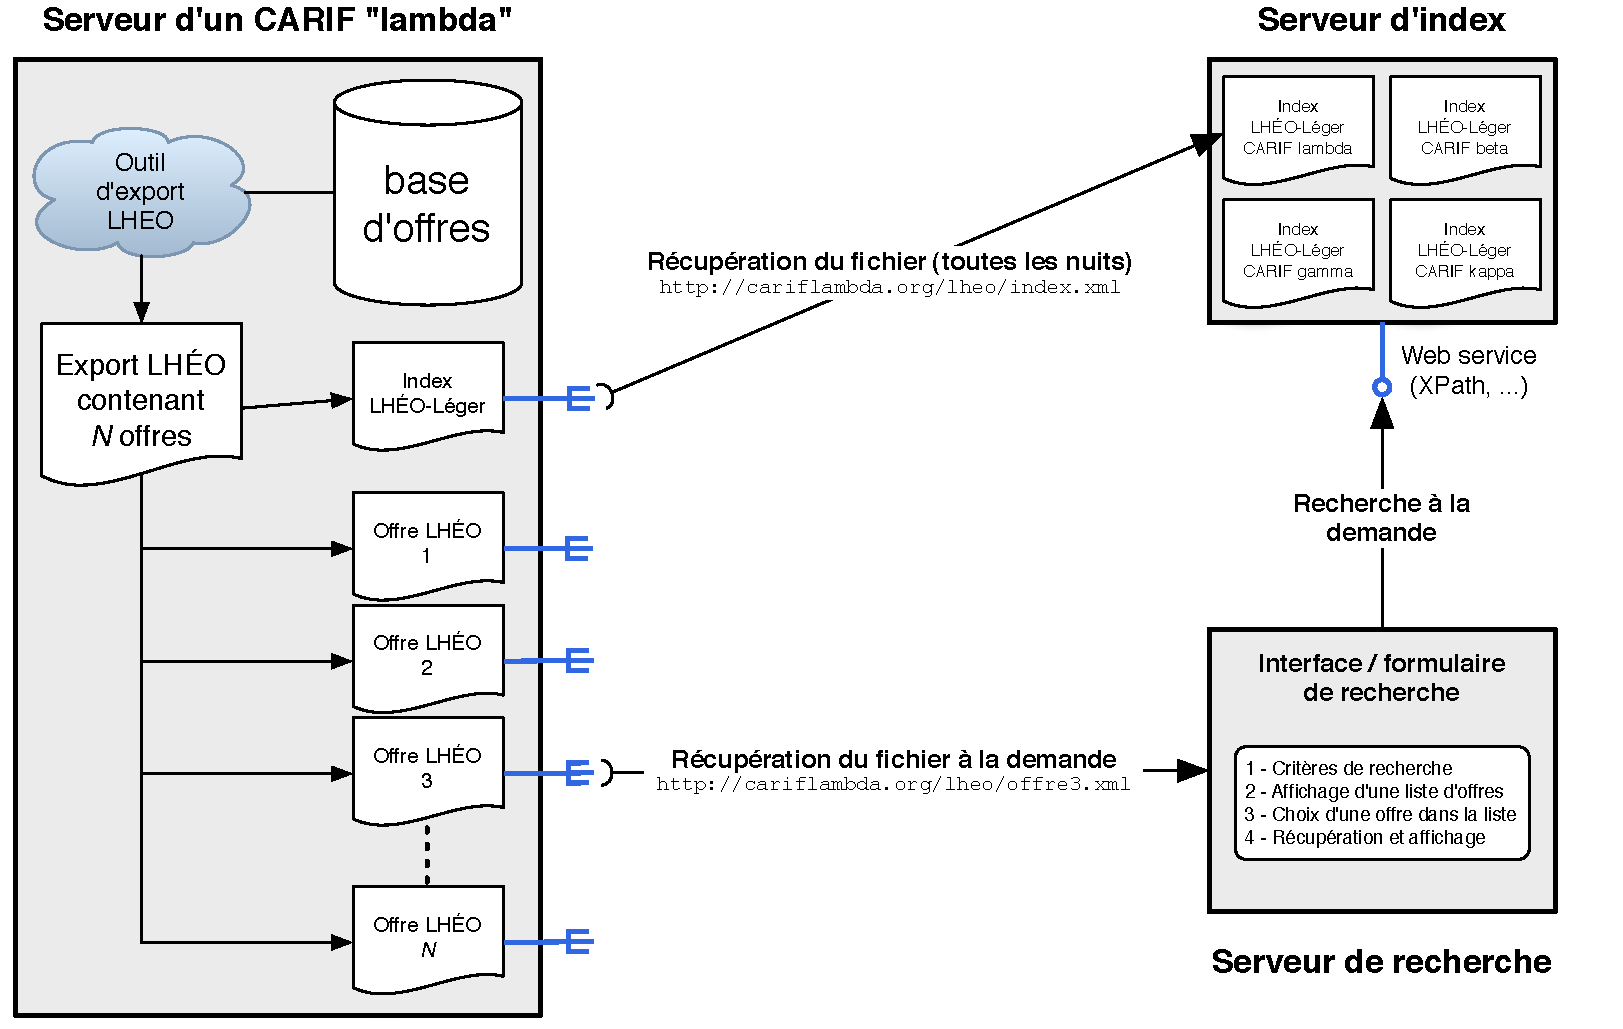
\includegraphics[width=\textwidth]{fonctionnement_recherche}$$
  \caption{\label{fig:recherche}exemple d'utilisation d'un résumé au format LHÉO-Index}
\end{figure}
    
\medskip
\noindent Voici les opérations effectuées par le \textbf{CARIF "lambda"}:

\begin{itemize} 
  
\item le CARIF "lambda" a une base d'offres dans un système de
  gestion de base de données (par exemple une base
  relationnelle). Régulièrement, un outil d'export permet
  d'extraire de cette base les offres au format LHÉO. Cet outil
  d'export est \textbf{spécifique} a une structure puisqu'il
  dépend du schéma des données utilisées dans la base;
  
\item chaque offre extraite de la base est déposée sur le
  serveur du CARIF à un emplacement spécifique. Chaque offre, au
  format XML LHÉO est accessible par l'intermédiaire d'une URL
  unique, comme par exemple:
  
  \begin{center}
\begin{verbatim}
http://cariflambda.org/lheo/offre3.xml
\end{verbatim}
  \end{center}
  
\item un index global, au format XML LHÉO-Index est créé
  contenant le résumé de toutes les offres disponibles sur le
  site. Cet index est disponible à une URL précise qui sera
  communiquée aux tiers qui pourrons l'exploiter, comme par
  exemple:
  
  \begin{center}
\begin{verbatim}
http://cariflambda.org/lheo/index.xml
\end{verbatim}
  \end{center}
  
\item chaque résumé d'offre (élément
  \texttt{<resume-offre>} de l'index en LHÉO-Index) contient
  dans l'attribut \texttt{file} l'URL de l'offre complète en
  format XML LHÉO disponible sur le serveur. Ainsi, en faisant une
  recherche dans l'index avec les informations résumées, il est
  possible d'accéder à la description complète de l'offre grâce à
  cette URL.
\end{itemize}

\medskip
\noindent Voici les opérations effectuées par le \textbf{serveur d'index}:

\begin{itemize} 
  
\item toutes les nuits (par exemple, d'autres modalités temporelles
  pourraient être définies), le fichier d'index au format XML
  LHÉO-Index est récupéré par le serveur d'index sur le site du
  \textbf{CARIF "lambda"}. L'emplacement (URL) de ce fichier d'index
  aura été transmis au préalable à l'administrateur du serveur d'index
  afin que celui-ci puisse configurer son application de
  récupération. Il est à noter que c'est la seule information de
  configuration que le CARIF a a transmettre au serveur d'index,
  l'emplacement de toutes les autres offres se trouvant dans le
  fichier d'index;

\item le serveur d'index récupère de la même façon sur d'autres CARIF
  des fichiers d'index;

\item le serveur d'index expose un \emph{service web} permettant à un
  serveur extérieur d'effectuer une recherche dans tous les index au
  format XML LHÉO-Index. Nous ne décrirons pas ici les modalités
  techniques de ce service web puisque la seule chose importante et
  qu'il permette de récupérer une liste d'offres correspondant à la
  recherche, chaque élément de la liste d'offres devant contenir l'URL
  permettant de récupérer l'offre complète sur le site du CARIF.
\end{itemize}

\medskip
\noindent Voici les opérations effectuées par le \textbf{serveur de recherche}:

\begin{itemize} 
\item le serveur de recherche présente à l'utilisateur une interface
  dans un navigateur web qui permet d'effectuer une recherche dans une
  base d'offre. L'utilisateur entre ses critères de recherche;
\item le serveur de recherche transforme les critères en une requête
  pour le service web du \textbf{serveur d'index} qui renvoie une
  liste d'offres répondant aux critères. Chaque offre contient l'URL
  de l'offre complète;
\item le serveur de recherche présente une liste des offres répondant
  aux critères, chaque offre étant représentée de manière résumée et
  succincte (l'information complète décrivant l'offre n'ayant pas
  encore été récupérée);
\item l'utilisateur peut choisir une offre de la liste;
\item lorsque l'utilisateur choisit une offre de la liste, le serveur
  de recherche récupère l'offre complète au format XML LHÉO sur le
  site du CARIF et affiche l'offre complète à l'utilisateur.
\end{itemize}
